\documentclass{article}
\usepackage{tikz}
\usetikzlibrary{automata,positioning}

\begin{document}

\begin{figure}[h]
    \centering
    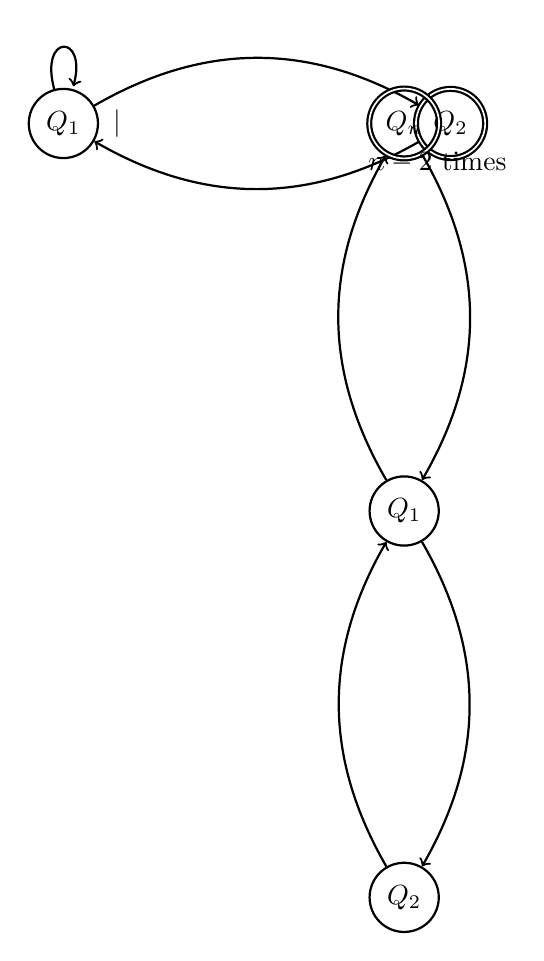
\begin{tikzpicture}[node distance=4cm,auto, thick,scale=1]
        \node[state]         (q_1)                  {$Q_1$};
        \draw[->,loop above] (q_1) edge node {} (q_1);
        
        \node[state, accepting, right=of q_1]         (q_2)                  {$Q_2$};
        \draw[->] (q_1) edge[bend left] node {} (q_2);
        \draw[->] (q_2) edge[bend left] node {} (q_1);
        
        \node [right=5mm] (sep) {$|$}; % separator between two sections
        
        \node[state, accepting, right=3cm of sep]         (qn)                  {$Q_n$};
        \node[state, below=of qn]     (q1) {$Q_1$};
        \node[state, below=of q1]     (q2) {$Q_2$};
        
        \draw[->] (q1) edge[bend left] node {} (qn);
        \draw[->] (qn) edge[bend left] node {} (q1);
        
        \draw[->] (q1) edge[bend left] node {} (q2);
        \draw[->] (q2) edge[bend left] node {} (q1);
        
        \node at (4.75, -0.5) {$n-2$ times};
    \end{tikzpicture}
    
    \begin{tabular}{@{}c@{}}
        $Q_i$ are elements of the state space. \\
        On the left, 1-cycles (which is an equilibrium) and a 2-cycle are frequently observed and behave deterministically. \\
        On the right, an $n$-cycle with $n > 2$ is never observed deterministically and stochastically will exist with probability 0.
    \end{tabular}
\end{figure}

\end{document}